\documentclass[aspectratio=169]{beamer}

% Shared Beamer settings for Applied Machine Learning lectures (UPES).
% Keep this file free of \documentclass to allow reuse via \input.

% Allow lecture sources to use shared theme/assets without copying them into each lecture folder.
% NOTE: These paths are relative to `Unit-xx/Lecture-yy/latex/` (and `Lab/Experiment-xx/latex/`).
\makeatletter
\def\input@path{{../../../_shared/}{../../../_shared/UPES-Beamer-Theme/}}
\makeatother

\usetheme{UPES}
\setbeamertemplate{navigation symbols}{}

\usepackage{amsmath}
\usepackage{amssymb}
\usepackage{booktabs}
\usepackage{graphicx}
\usepackage{hyperref}
\usepackage{xcolor}
\usepackage{listings}

% Code listings (Python-oriented for this subject).
\lstset{
  language=Python,
  basicstyle=\ttfamily\small,
  keywordstyle=\color{blue},
  commentstyle=\color{gray},
  stringstyle=\color{teal},
  showstringspaces=false,
  columns=fullflexible,
  breaklines=true
}

\usepackage{tikz}
\usetikzlibrary{arrows.meta,positioning,shapes.geometric,calc,fit,backgrounds}

% Per-slide source line (references shown on the slide itself).
\newcommand{\slidesources}[1]{%
  \vfill
  {\tiny\color{gray}\raggedright\sloppy\parbox{\linewidth}{Sources: #1}\par}%
}

% Unit-wise source strings for this subject (used by slides/notes).
% Path is relative to the lecture `latex/` folder (the compilation CWD).
% Source strings for Applied Machine Learning (CSAI2017P) — used by slides + notes.
% Prescribed texts and reference books are taken from the course syllabus.
% Support texts are the author-hosted open-access editions:
%   statlearning.com            (ISL with Python)
%   probml.github.io/pml-book   (Murphy, Probabilistic Machine Learning)
%   d2l.ai                      (Dive into Deep Learning)
%   mml-book.github.io          (Mathematics for Machine Learning)

\newcommand{\AMLRepoURL}{https://github.com/tali7c/Applied-Machine-Learning}

% --- prescribed -------------------------------------------------------------
\newcommand{\AMLPrescribed}{%
M\"uller and Guido, \textit{Introduction to Machine Learning with Python}, O'Reilly, 2016.;%
Bishop, \textit{Pattern Recognition and Machine Learning}, Springer, 2006.;%
Murphy, \textit{Machine Learning: A Probabilistic Perspective}, MIT Press, 2012.;%
Han, Kamber and Pei, \textit{Data Mining: Concepts and Techniques} (3e), Morgan Kaufmann, 2012.%
}

% --- unit-wise ---------------------------------------------------------------
\newcommand{\AMLUnitISources}{%
M\"uller and Guido, \textit{Introduction to Machine Learning with Python}, Ch. 1.;%
Bishop, \textit{Pattern Recognition and Machine Learning}, Ch. 1.;%
Murphy, \textit{Probabilistic Machine Learning: An Introduction}, MIT Press, 2022, Ch. 1.;%
Mitchell, \textit{Machine Learning}, McGraw Hill, 1997, Ch. 1.;%
Scikit-learn documentation, accessed 2026-08-04.%
}

\newcommand{\AMLUnitIISources}{%
Bishop, \textit{Pattern Recognition and Machine Learning}, \S1.5, \S4.3, \S7.1.;%
Zhang, Lipton, Li and Smola, \textit{Dive into Deep Learning}, \S3.4.;%
Shalev-Shwartz and Ben-David, \textit{Understanding Machine Learning}, Ch. 15.;%
Murphy, \textit{Probabilistic Machine Learning: An Introduction}, Ch. 5.%
}

\newcommand{\AMLUnitIIISources}{%
Zhang, Lipton, Li and Smola, \textit{Dive into Deep Learning}, Ch. 12 (Optimization Algorithms).;%
Deisenroth, Faisal and Ong, \textit{Mathematics for Machine Learning}, Ch. 7.;%
Kingma and Ba, ``Adam: A Method for Stochastic Optimization,'' ICLR 2015.;%
Ruder, ``An overview of gradient descent optimization algorithms,'' arXiv:1609.04747, 2016.%
}

\newcommand{\AMLUnitIVSources}{%
Han, Kamber and Pei, \textit{Data Mining: Concepts and Techniques} (3e), Ch. 3.;%
M\"uller and Guido, \textit{Introduction to Machine Learning with Python}, Ch. 3--4.;%
James, Witten, Hastie, Tibshirani and Taylor, \textit{An Introduction to Statistical Learning with Python}, Ch. 5--6, 12.;%
Scikit-learn documentation (preprocessing, model selection), accessed 2026-08-04.%
}

\newcommand{\AMLUnitVSources}{%
James et al., \textit{An Introduction to Statistical Learning with Python}, Ch. 3--6.;%
Bishop, \textit{Pattern Recognition and Machine Learning}, Ch. 3.;%
Deisenroth, Faisal and Ong, \textit{Mathematics for Machine Learning}, Ch. 9.;%
M\"uller and Guido, \textit{Introduction to Machine Learning with Python}, \S2.3.%
}

\newcommand{\AMLUnitVISources}{%
Han, Kamber and Pei, \textit{Data Mining: Concepts and Techniques} (3e), Ch. 8--9.;%
James et al., \textit{An Introduction to Statistical Learning with Python}, Ch. 8--9.;%
Bishop, \textit{Pattern Recognition and Machine Learning}, Ch. 4--5, 7, 14.;%
Zhang et al., \textit{Dive into Deep Learning}, Ch. 5.%
}

\newcommand{\AMLUnitVIISources}{%
Han, Kamber and Pei, \textit{Data Mining: Concepts and Techniques} (3e), Ch. 10.;%
James et al., \textit{An Introduction to Statistical Learning with Python}, Ch. 12.;%
M\"uller and Guido, \textit{Introduction to Machine Learning with Python}, \S3.5.;%
Ester, Kriegel, Sander and Xu, ``A density-based algorithm for discovering clusters (DBSCAN),'' KDD 1996.%
}

\newcommand{\AMLLabSources}{%
M\"uller and Guido, \textit{Introduction to Machine Learning with Python}, companion notebooks.;%
McKinney, \textit{Python for Data Analysis} (3e), O'Reilly, 2022.;%
Scikit-learn user guide, accessed 2026-08-04.;%
Matplotlib and Seaborn documentation, accessed 2026-08-04.%
}



\graphicspath{{../figures/}{../images/}{../../../_shared/}{../../../_shared/UPES-Beamer-Theme/}}

\title[Applied Machine Learning]{Applied Machine Learning}
\subtitle{Unit 05 -- Lecture 08: Regression Foundations and Least Squares}
\author{Tofik Ali}
\institute{School of Computer Science, UPES Dehradun}
\date{Autumn 2026}

% ---- a compact "output" block so code and its result sit together ----------
\lstdefinestyle{outblk}{
  basicstyle=\ttfamily\scriptsize\color{black!75},
  backgroundcolor=\color{black!5}, frame=leftline, framerule=2pt,
  rulecolor=\color{black!30}, breaklines=true, columns=fullflexible,
  keepspaces=true,   % several outputs below are aligned tables
  language={},       % printed output is not Python: do not syntax-highlight it
  xleftmargin=4pt, aboveskip=1pt, belowskip=1pt, literate={-}{{-}}1}
\lstnewenvironment{outblk}{\lstset{style=outblk}}{}

\begin{document}

\UPESCoverFrame
\setcounter{framenumber}{0}

\begin{frame}[shrink=5]
  \titlepage
  \begin{center}
    \footnotesize Topic focus: \textbf{for this one model, the minimisation
    has an answer you can write down}\\[0.2em]
    \footnotesize Repository: \texttt{\AMLRepoURL}
  \end{center}
  \slidesources{\AMLUnitVSources}
\end{frame}

\begin{frame}{Quick Links}
  \centering
  \hyperlink{sec:intro}{\beamerbutton{What regression is}}\hspace{0.4em}
  \hyperlink{sec:models}{\beamerbutton{Models}}\hspace{0.4em}
  \hyperlink{sec:steps}{\beamerbutton{Steps}}\hspace{0.4em}
  \hyperlink{sec:slr}{\beamerbutton{Simple linear regression}}\hspace{0.4em}
  \hyperlink{sec:derive}{\beamerbutton{The derivation}}\\[0.6em]
  \hyperlink{sec:hand}{\beamerbutton{Five points}}\hspace{0.4em}
  \hyperlink{sec:props}{\beamerbutton{Line of best fit}}\hspace{0.4em}
  \hyperlink{sec:matrix}{\beamerbutton{Matrix form}}\hspace{0.4em}
  \hyperlink{sec:gd}{\beamerbutton{Two roads}}\hspace{0.4em}
  \hyperlink{sec:caution}{\beamerbutton{Cautions}}\hspace{0.4em}
  \hyperlink{sec:summary}{\beamerbutton{Summary}}
\end{frame}

\begin{frame}{Agenda}
  \tableofcontents
\end{frame}

\begin{frame}[shrink=6]{How this lecture works}
  \begin{columns}[T]
    \begin{column}{0.48\textwidth}
      \begin{block}{Every idea appears twice}
        \begin{enumerate}
          \item \textbf{By hand} --- five points, $x = 1,2,3,4,5$. Every
            intermediate quantity is an integer or a clean decimal, so the
            whole fit goes on paper.
          \item \textbf{In code} --- \texttt{np.polyfit},
            \texttt{LinearRegression} and $(X^{\!\top}\!X)^{-1}X^{\!\top}y$
            on the same five numbers, then on $442$ real patients.
        \end{enumerate}
      \end{block}
    \end{column}
    \begin{column}{0.48\textwidth}
      \begin{alertblock}{Commit before you look}
        Six slides ask you to predict a number before it appears. Write your
        guess down. Being wrong on paper is how the idea sticks.
      \end{alertblock}
    \end{column}
  \end{columns}
  \vspace{0.3em}
  \begin{center}
    \small The centrepiece is \textbf{a derivation}: two partial derivatives
    set to zero, solved, giving $b_1 = S_{xy}/S_{xx}$ and
    $b_0 = \bar y - b_1\bar x$. It is examinable, and we do it on the board.
  \end{center}
\end{frame}

\begin{frame}[shrink=5]{Where we are}
  \begin{columns}[T]
    \begin{column}{0.47\textwidth}
      \begin{block}{Unit II said \emph{what} to minimise}
        The mean squared error
        $J(w) = \frac1n\sum_i (\hat y_i - y_i)^2$. A number that says how
        wrong a model is.
      \end{block}
      \begin{block}{Unit III said \emph{how} to minimise it}
        Gradient descent, and its stochastic, mini-batch, momentum and
        adaptive relatives. Take a step downhill; repeat.
      \end{block}
      \begin{block}{Unit IV made the table fit to use}
        Cleaned, scaled, encoded, reduced, split.
      \end{block}
    \end{column}
    \begin{column}{0.49\textwidth}
      \begin{exampleblock}{Unit V asks a new question}
        Take the simplest possible model --- a straight line --- and the same
        squared-error objective. \textbf{Do we actually need to iterate?}
      \end{exampleblock}
      \begin{alertblock}{The answer, for today only}
        No. Setting two derivatives to zero gives two linear equations in two
        unknowns, and \textbf{you solve them once}. We will then run gradient
        descent on the same data and watch it crawl to exactly the number the
        formula produced in one line.
      \end{alertblock}
    \end{column}
  \end{columns}
\end{frame}

\begin{frame}{One seed, and every number in this deck reproduces}
  \begin{columns}[T]
    \begin{column}{0.48\textwidth}
      \begin{block}{The data}
        \small Bundled \texttt{load\_diabetes},
        \texttt{load\_breast\_cancer} and \texttt{load\_wine}, the published
        Anscombe table, and the five-point revision example. Nothing is
        downloaded, and none of it is randomly generated.
      \end{block}
    \end{column}
    \begin{column}{0.48\textwidth}
      \begin{block}{The randomness}
        \small One seed for the whole lecture:
        \texttt{np.random.default\_rng(0)}, and \texttt{random\_state=0} on
        every split and every stochastic estimator. Each listing that draws or
        shuffles shows it.
      \end{block}
    \end{column}
  \end{columns}
  \vspace{0.5em}
  \begin{exampleblock}{Why this matters to you}
    \centering\small
    Every number in this deck is printed by one script. Run the code as
    written and you get the same numbers --- which is the only reason to
    believe a number on a slide.
  \end{exampleblock}
\end{frame}

% =====================================================================
\section[Regression]{What regression is}
\label{sec:intro}

\begin{frame}[shrink=6]{Regression: predicting a number}
  \begin{exampleblock}{}
    \centering\large
    Modelling how a \textbf{quantitative} response varies with one or more
    predictors.
  \end{exampleblock}
  \vspace{0.3em}
  \begin{columns}[T]
    \begin{column}{0.49\textwidth}
      \begin{block}{The vocabulary, which the exam uses}
        \small
        \begin{tabular}{@{}ll@{}}
          $y$ & response, dependent, target\\
          $x$ & predictor, regressor, feature\\
          $\varepsilon$ & error, disturbance, noise\\
        \end{tabular}\\[0.3em]
        The model splits $y$ into a \textbf{systematic} part $f(x)$ and a
        \textbf{random} part $\varepsilon$:
        \[ y = f(x) + \varepsilon. \]
      \end{block}
    \end{column}
    \begin{column}{0.47\textwidth}
      \begin{alertblock}{Regression against classification}
        \small $y$ continuous $\Rightarrow$ regression; $y$ a label
        $\Rightarrow$ classification. Rupees, marks, temperature, disease
        progression are regression. Spam / not spam is not.
      \end{alertblock}
      \begin{block}{And the word itself}
        \small Galton, 1886: tall fathers have sons who are tall but
        \emph{less so} --- ``regression towards mediocrity''. The name stuck
        to the method, not the phenomenon.
      \end{block}
    \end{column}
  \end{columns}
\end{frame}

\begin{frame}[shrink=6]{Two jobs a regression can do}
  \begin{columns}[T]
    \begin{column}{0.48\textwidth}
      \begin{block}{Prediction}
        Given a new $x$, what is $y$? Nobody has to understand the model.
        Judge it by held-out error.\\[0.3em]
        \small \emph{What will this flat sell for?}
      \end{block}
    \end{column}
    \begin{column}{0.48\textwidth}
      \begin{exampleblock}{Explanation}
        Which predictors matter, in which direction, by how much? Judge it by
        whether the coefficients can be trusted.\\[0.3em]
        \small \emph{Does an extra hour of revision raise the mark, and by
        how much?}
      \end{exampleblock}
    \end{column}
  \end{columns}
  \vspace{0.3em}
  \begin{alertblock}{The two jobs pull in different directions}
    A model can predict well with coefficients that mean nothing --- Lecture 6
    showed exactly that with the dummy variable trap, where two completely
    different coefficient vectors gave \emph{identical} predictions.
    \textbf{Decide which job you are doing before you choose the model.}
  \end{alertblock}
  \begin{center}\small
    Today's model does both, which is why it is still the first one taught.
  \end{center}
\end{frame}

\begin{frame}[shrink=8]{Where regression is actually used}
  \begin{center}\small
  \begin{tabular}{@{}lll@{}}
    \toprule
    \textbf{Field} & \textbf{Response $y$} & \textbf{Predictors $x$}\\
    \midrule
    Medicine & disease progression in a year & BMI, blood pressure, six serum
      measures\\
    Real estate & sale price, in rupees & area, rooms, age, locality\\
    Energy & tomorrow's peak load & temperature, weekday, last week's load\\
    Agriculture & yield per hectare & rainfall, fertiliser, soil nitrogen\\
    Manufacturing & tensile strength & alloy fractions, furnace temperature\\
    Finance & next-day return & yesterday's return, volume, volatility\\
    Education & end-semester mark & attendance, internal marks, hours studied\\
    \bottomrule
  \end{tabular}
  \end{center}
  \vspace{0.3em}
  \begin{block}{The one we will use all lecture}
    \small \texttt{load\_diabetes}: $442$ patients, $10$ measurements, and a
    quantitative score of disease progression one year after baseline. It
    ships with scikit-learn, so \textbf{nothing downloads}.
  \end{block}
\end{frame}

% =====================================================================
\section[Models]{Regression examples and models}
\label{sec:models}

\begin{frame}[shrink=7]{The family of regression models}
  \begin{center}\small
  \begin{tabular}{@{}lll@{}}
    \toprule
    \textbf{Model} & \textbf{Form} & \textbf{Fitted by}\\
    \midrule
    Simple linear & $y = \beta_0 + \beta_1 x + \varepsilon$ &
      least squares, closed form\\
    Multiple linear & $y = \beta_0 + \sum_j \beta_j x_j + \varepsilon$ &
      least squares, closed form (L11)\\
    Polynomial & $y = \beta_0 + \beta_1 x + \beta_2 x^2 + \dots$ &
      least squares, closed form\\
    Log / reciprocal terms & $y = \beta_0 + \beta_1 \log x + \varepsilon$ &
      least squares, closed form\\
    \midrule
    Ridge, lasso & least squares $+$ a penalty & closed form / convex
      solver (L12)\\
    Logistic & $\Pr(y=1) = \sigma(\beta_0 + \beta_1x)$ &
      maximum likelihood, iterative (L10)\\
    Nonlinear & $y = \theta_1 e^{-\theta_2 x} + \varepsilon$ &
      numerical optimisation\\
    Nonparametric & trees, $k$-NN, splines & no global equation\\
    \bottomrule
  \end{tabular}
  \end{center}
  \vspace{0.2em}
  \begin{alertblock}{The dividing line is not curvature. It is the parameters}
    \small A model is \textbf{linear} when it is linear \emph{in the
    parameters}. $y = \beta_0 + \beta_1 x + \beta_2 x^2$ draws a parabola and
    is a linear model. $y = \beta_0 + \beta_0\beta_1 x$ draws a straight line
    and is \emph{not}.
  \end{alertblock}
\end{frame}

\begin{frame}[shrink=8]{Drawn: four models, one fitting method between them}
  \begin{center}
    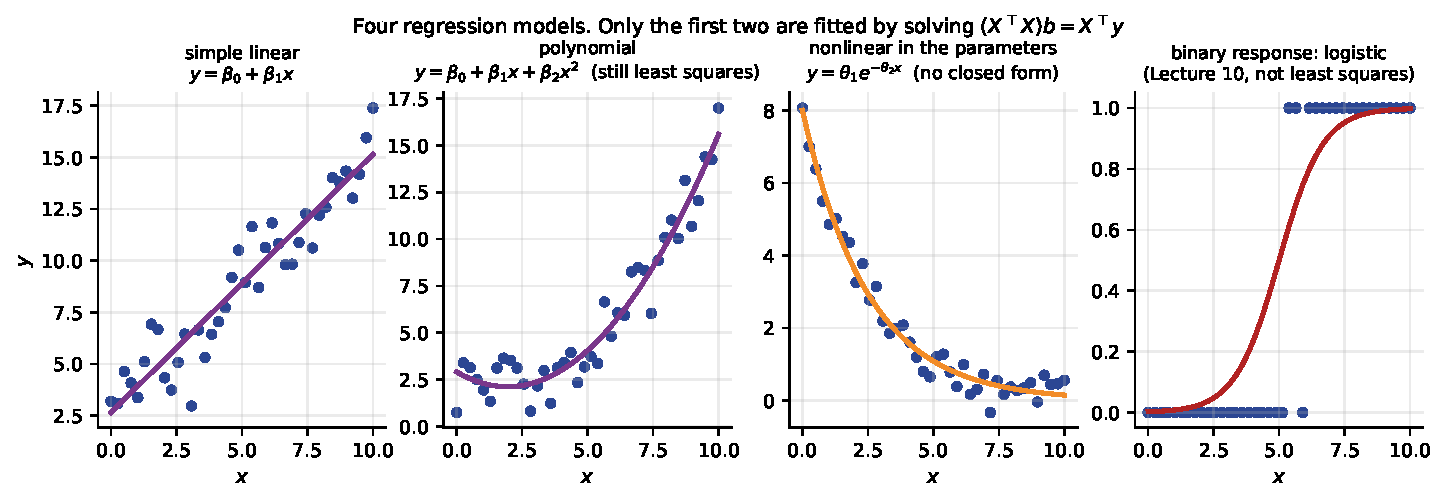
\includegraphics[width=0.98\textwidth]{models.pdf}
  \end{center}
  \begin{center}\small
    Panels 1 and 2 are both solved by $(X^{\!\top}\!X)b = X^{\!\top}y$; only
    the columns of $X$ differ. Panel 3 has a parameter inside an exponential
    and needs an iterative solver. Panel 4 has a $0/1$ response, so squared
    error is the wrong objective altogether --- that is Lecture 10.
  \end{center}
\end{frame}

\begin{frame}[fragile,shrink=7]{The same normal equations, three different designs}
Fit degree $1$, $2$ and $3$ to the \emph{same} $40$ points, each time by
solving $(X^{\!\top}\!X)b = X^{\!\top}y$:
\begin{lstlisting}
P = np.column_stack([xp**k for k in range(deg + 1)])   # the design matrix
bhat = np.linalg.solve(P.T @ P, P.T @ yp)              # the normal equations
\end{lstlisting}
\begin{outblk}
degree 1  design (40, 2)  coefficients [ 4.4626 -0.4485]                  SSE 265.953
degree 2  design (40, 3)  coefficients [ 1.7027 -0.4485  0.8751]          SSE  22.655
degree 3  design (40, 4)  coefficients [ 1.7027 -0.4331  0.8751 -0.0027]  SSE  22.649
\end{outblk}
\onslide<2->
\begin{center}\small
  Data generated from $y = 2 - 0.5x + 0.8x^2 + \varepsilon$. \textbf{One
  solver, three models.} Everything in this lecture about the straight line
  transfers, unchanged, to any design matrix --- which is why we spend the
  time on it.
\end{center}
\end{frame}

% =====================================================================
\section[Steps]{Steps in a regression analysis}
\label{sec:steps}

\begin{frame}[shrink=7]{The eight steps}
  \begin{columns}[T]
    \begin{column}{0.52\textwidth}
      \begin{enumerate}\small
        \item \textbf{Statement of the problem.} What question, in words,
          before any data.
        \item \textbf{Selection of variables.} What is $y$, what could be
          $x$, in what units.
        \item \textbf{Data collection.} How many rows, how gathered, how
          split.
        \item \textbf{Model specification.} Write the equation down.
        \item \textbf{Choice of fitting method.} Least squares, maximum
          likelihood, penalised least squares.
        \item \textbf{Fitting.} Compute the estimates.
        \item \textbf{Model validation.} Residuals, held-out error,
          assumptions.
        \item \textbf{Use.} Predict, or interpret --- and say which.
      \end{enumerate}
    \end{column}
    \begin{column}{0.44\textwidth}
      \begin{alertblock}{Steps 1--3 are where analyses die}
        \small By the time you type \texttt{fit()} the important decisions
        are already made. A perfect fit to the wrong response answers the
        wrong question perfectly.
      \end{alertblock}
      \begin{block}{And step 7 sends you back}
        \small Validation is not a rubber stamp. If the residuals show
        structure you return to step 4, not to step 6. That loop is
        Lecture 9's subject.
      \end{block}
    \end{column}
  \end{columns}
\end{frame}

\begin{frame}[fragile,shrink=7]{All eight steps, once, on real patients}
\begin{outblk}
1 problem   : does body mass index predict disease progression?
2 variables : y = progression score; x = bmi (centred and scaled here)
3 data      : 442 patients, 331 train / 111 test
4 model     : y = b0 + b1 x + e
5 method    : least squares
6 fit       : LinearRegression  b0 = 153.2257  b1 = 1016.9235
              by hand           b0 = 153.2257  b1 = 1016.9235
7 check     : train RMSE 61.711   test RMSE 64.664
              training residuals sum to 2.274e-12
              5-fold RMSE 62.605 +/- 2.888
              always predicting ybar gives RMSE 77.006
8 use       : one sd more bmi predicts 49.4 more progression points
\end{outblk}
\onslide<2->
\begin{center}\small
  Read line 7 twice. \textbf{$62.6$ against $77.0$}: one column of one
  measurement removes about a fifth of the error of guessing the mean, and
  the test RMSE is close to the training RMSE, so nothing is over-fitted.
  Read line 6 too --- \textbf{the library and the hand formula agree to four
  decimals}, which is the whole point of the next twenty minutes.
\end{center}
\end{frame}

\begin{frame}[shrink=8]{Drawn: step 7, on the same fit}
  \begin{center}
    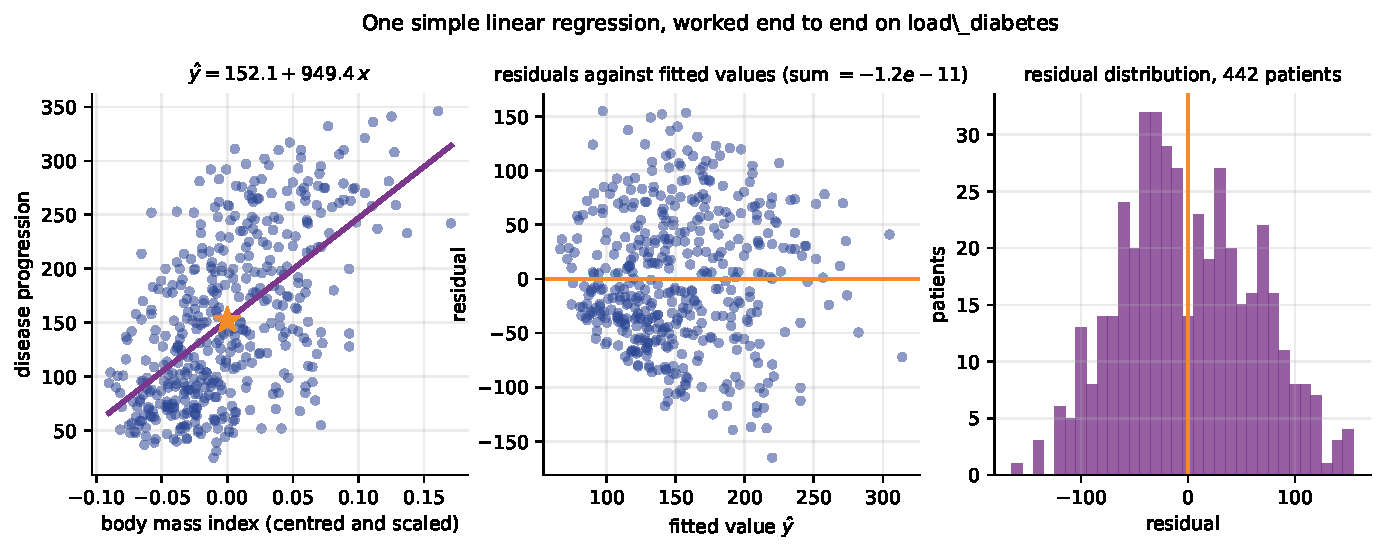
\includegraphics[width=0.98\textwidth]{diabetes.pdf}
  \end{center}
  \begin{center}\small
    Left: the fitted line passes through the star, which is
    $(\bar x, \bar y)$ --- we prove that in twenty minutes. Middle: residuals
    against fitted values, summing to $10^{-11}$; we prove that too. Right:
    they are roughly symmetric about zero, which is the assumption Lecture 9
    will lean on. \textbf{The spread does widen to the right, and that is a
    real defect of this model.}
  \end{center}
\end{frame}

% =====================================================================
\section[SLR]{Simple linear regression}
\label{sec:slr}

\begin{frame}[shrink=6]{The model, stated properly}
  \begin{exampleblock}{}
    \centering\large
    $y_i = \beta_0 + \beta_1 x_i + \varepsilon_i, \qquad i = 1,\dots,n$
  \end{exampleblock}
  \vspace{0.2em}
  \begin{columns}[T]
    \begin{column}{0.5\textwidth}
      \begin{block}{Four assumptions}
        \small
        \begin{enumerate}
          \item \textbf{Linearity}: $\mathbb{E}[y \mid x] = \beta_0 +
            \beta_1 x$.
          \item \textbf{Independence}: the $\varepsilon_i$ are independent.
          \item \textbf{Constant variance}: $\mathrm{Var}(\varepsilon_i) =
            \sigma^2$, the same for every $x$.
          \item \textbf{Zero mean}: $\mathbb{E}[\varepsilon_i] = 0$.
        \end{enumerate}
      \end{block}
    \end{column}
    \begin{column}{0.47\textwidth}
      \begin{alertblock}{Two lines, and do not confuse them}
        \small $\beta_0, \beta_1$ describe the \textbf{population} and you
        will never see them.\\[0.25em]
        $b_0, b_1$ are \textbf{estimates} computed from your $n$ rows, and
        they change if you collect the data again.
      \end{alertblock}
      \begin{block}{Notation for the rest of the lecture}
        \small $\hat y_i = b_0 + b_1 x_i$ is the fitted value;
        $e_i = y_i - \hat y_i$ is the residual. $\varepsilon_i$ is
        unobservable, $e_i$ is on your screen.
      \end{block}
    \end{column}
  \end{columns}
\end{frame}

\begin{frame}[shrink=6]{Which line? We must choose a criterion}
  \begin{columns}[T]
    \begin{column}{0.48\textwidth}
      \begin{block}{Candidate criteria}
        \small
        \begin{itemize}
          \item minimise $\sum_i e_i$ --- \textbf{useless}: positive and
            negative errors cancel, and infinitely many lines score zero.
          \item minimise $\sum_i |e_i|$ --- sensible, robust, and has
            \emph{no closed form}.
          \item minimise $\max_i |e_i|$ --- lets one bad row dictate the
            whole line.
          \item minimise $\sum_i e_i^2$ --- \textbf{least squares}.
        \end{itemize}
      \end{block}
    \end{column}
    \begin{column}{0.48\textwidth}
      \begin{exampleblock}{Why squares win}
        \small
        \begin{enumerate}
          \item Differentiable everywhere, so calculus applies.
          \item The derivative is \emph{linear} in $b_0, b_1$, so the
            stationary condition is a linear system.
          \item Convex, so the stationary point is the global minimum.
          \item Under Normal noise it is also the maximum-likelihood answer
            --- Lecture 9.
        \end{enumerate}
      \end{exampleblock}
    \end{column}
  \end{columns}
  \vspace{0.2em}
  \begin{center}\small
    And one honest cost: squaring makes the criterion \textbf{sensitive to
    outliers}, which we measure later in the lecture.
  \end{center}
\end{frame}

\begin{frame}[shrink=8]{Drawn: why squares, and what absolutes cost you}
  \begin{center}
    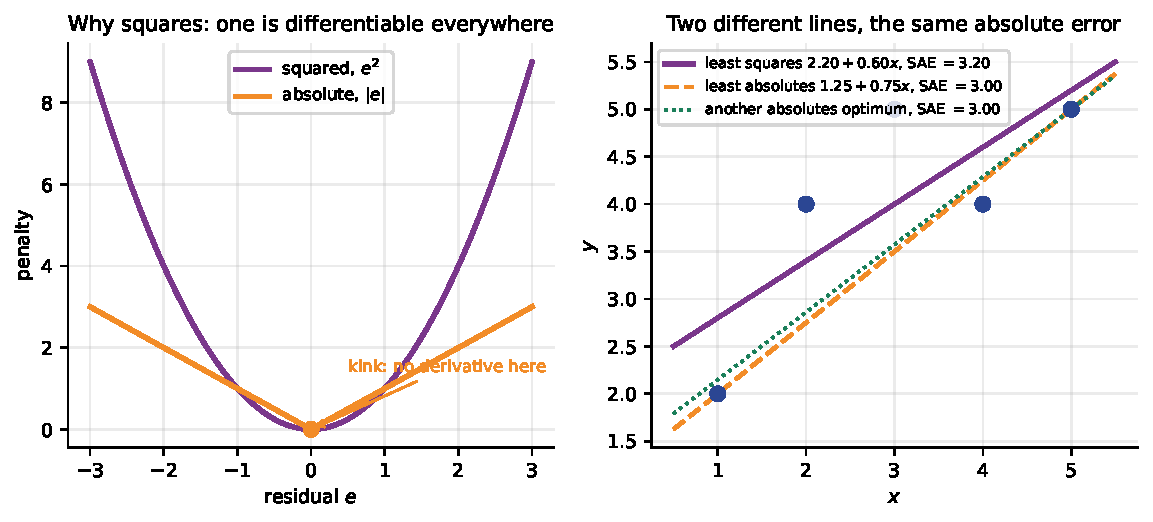
\includegraphics[width=0.92\textwidth]{lossshape.pdf}
  \end{center}
  \begin{center}\small
    Left: $|e|$ has a corner at $e=0$ and no derivative there, so ``set the
    derivative to zero'' is not available. Right: on our five points the two
    dashed lines have \textbf{exactly the same} total absolute error
    ($3.00$), so the least-absolute-deviation answer is \emph{not unique}.
    Least squares has one answer, always.
  \end{center}
\end{frame}

% =====================================================================
\section[Derivation]{Least-squares estimation: the derivation}
\label{sec:derive}

\begin{frame}[shrink=5]{The object we are minimising}
  For a given pair $(b_0, b_1)$ the total squared error is
  \[
    \mathrm{SSE}(b_0, b_1) \;=\; \sum_{i=1}^{n}\bigl(y_i - b_0 -
      b_1 x_i\bigr)^2 .
  \]
  \begin{block}{Two things to notice before differentiating}
    \begin{itemize}
      \item $x_i$ and $y_i$ are \textbf{known numbers}. The unknowns are
        $b_0$ and $b_1$ --- two of them, not $n$.
      \item Each term is a square, so $\mathrm{SSE} \ge 0$: the surface is a
        bowl. It has a bottom, and we are about to find it exactly.
    \end{itemize}
  \end{block}
  \begin{alertblock}{This is the L3 objective, up to a constant}
    $J(w) = \frac1n\lVert Xw - y\rVert^2 = \frac1n\,\mathrm{SSE}$. Dividing
    by $n$ does not move the minimiser. \textbf{Same function, same answer,
    two ways of getting there.}
  \end{alertblock}
\end{frame}

\begin{frame}[shrink=4]{Step 1: the two partial derivatives}
  Differentiate term by term, using the chain rule on
  $(y_i - b_0 - b_1x_i)^2$:
  \begin{align*}
    \frac{\partial\,\mathrm{SSE}}{\partial b_0}
      &= \sum_{i=1}^{n} 2\bigl(y_i - b_0 - b_1x_i\bigr)\cdot(-1)
       = -2\sum_{i=1}^{n}\bigl(y_i - b_0 - b_1x_i\bigr),\\[0.3em]
    \frac{\partial\,\mathrm{SSE}}{\partial b_1}
      &= \sum_{i=1}^{n} 2\bigl(y_i - b_0 - b_1x_i\bigr)\cdot(-x_i)
       = -2\sum_{i=1}^{n} x_i\bigl(y_i - b_0 - b_1x_i\bigr).
  \end{align*}
  \begin{center}\small
    The bracket is exactly the residual $e_i$. So the two derivatives are
    $-2\sum e_i$ and $-2\sum x_i e_i$ --- remember that; it gives us two
    properties of the fitted line for free.
  \end{center}
\end{frame}

\begin{frame}[shrink=4]{Step 2: set both to zero --- the normal equations}
  Dividing by $-2$ and expanding:
  \begin{align*}
    \sum_i y_i - n b_0 - b_1\sum_i x_i &= 0
      &&\Longrightarrow&& \;n\,b_0 + b_1\sum_i x_i = \sum_i y_i,\\
    \sum_i x_iy_i - b_0\sum_i x_i - b_1\sum_i x_i^2 &= 0
      &&\Longrightarrow&& \;b_0\sum_i x_i + b_1\sum_i x_i^2 = \sum_i x_iy_i .
  \end{align*}
  \begin{exampleblock}{Two linear equations in two unknowns}
    \centering
    These are the \textbf{normal equations}. Every quantity in them ---
    $n$, $\sum x_i$, $\sum y_i$, $\sum x_i^2$, $\sum x_iy_i$ --- is a number
    you can read off the data in one pass.
  \end{exampleblock}
  \begin{center}\small
    Notice what has happened: a minimisation over a continuum of lines has
    become \textbf{a system of two linear equations}. That is the whole
    trick, and it is available because the derivative of a square is linear.
  \end{center}
\end{frame}

\begin{frame}[shrink=4]{Step 3: solve them}
  Divide the first equation by $n$:
  \[
    b_0 + b_1 \bar x = \bar y
    \qquad\Longrightarrow\qquad
    \boxed{\,b_0 = \bar y - b_1 \bar x\,}
  \]
  Substitute into the second and collect the $b_1$ terms:
  \[
    (\bar y - b_1\bar x)\sum_i x_i + b_1 \sum_i x_i^2 = \sum_i x_iy_i
    \;\Longrightarrow\;
    b_1\Bigl(\sum_i x_i^2 - \bar x \sum_i x_i\Bigr)
      = \sum_i x_iy_i - \bar y\sum_i x_i .
  \]
  Using $\sum_i x_i = n\bar x$, the two brackets are
  $\sum x_i^2 - n\bar x^2$ and $\sum x_iy_i - n\bar x\bar y$, which are
  exactly
  \[
    S_{xx} = \sum_i (x_i-\bar x)^2, \qquad
    S_{xy} = \sum_i (x_i-\bar x)(y_i-\bar y),
  \]
  \begin{exampleblock}{}
    \centering\large
    $\displaystyle b_1 = \frac{S_{xy}}{S_{xx}}, \qquad
      b_0 = \bar y - b_1\bar x$
  \end{exampleblock}
\end{frame}

\begin{frame}[shrink=6]{Why those two brackets really are $S_{xx}$ and $S_{xy}$}
  This expansion is worth doing once, because it appears in every regression
  proof you will meet:
  \begin{align*}
    \sum_i (x_i - \bar x)^2
      &= \sum_i x_i^2 - 2\bar x\sum_i x_i + n\bar x^2
       = \sum_i x_i^2 - 2n\bar x^2 + n\bar x^2
       = \sum_i x_i^2 - n\bar x^2,\\[0.3em]
    \sum_i (x_i-\bar x)(y_i-\bar y)
      &= \sum_i x_iy_i - \bar y\sum_i x_i - \bar x\sum_i y_i + n\bar x\bar y
       = \sum_i x_iy_i - n\bar x\bar y .
  \end{align*}
  \begin{block}{Two forms of the same number}
    \small The left-hand forms are numerically safer; the right-hand forms
    are what you use in an examination, because $\sum x_i$, $\sum x_i^2$ and
    $\sum x_iy_i$ come straight out of a table of five rows.
  \end{block}
\end{frame}

\begin{frame}[shrink=4]{Step 4: is it a minimum? The second-order condition}
  A stationary point could be a minimum, a maximum or a saddle. Take the
  second derivatives:
  \[
    \frac{\partial^2 \mathrm{SSE}}{\partial b_0^2} = 2n,\qquad
    \frac{\partial^2 \mathrm{SSE}}{\partial b_1^2} = 2\sum_i x_i^2,\qquad
    \frac{\partial^2 \mathrm{SSE}}{\partial b_0\,\partial b_1} =
      2\sum_i x_i .
  \]
  \[
    H = 2\begin{pmatrix} n & \sum_i x_i\\[2pt] \sum_i x_i & \sum_i x_i^2
      \end{pmatrix},
    \qquad
    \det H = 4\Bigl(n\sum_i x_i^2 - \bigl(\textstyle\sum_i x_i\bigr)^2\Bigr)
           = 4n\,S_{xx}.
  \]
  \begin{exampleblock}{}
    \centering
    $H_{11} = 2n > 0$ and $\det H = 4nS_{xx} > 0$ whenever the $x_i$ are not
    all equal. \textbf{So $H$ is positive definite, SSE is strictly convex,
    and the stationary point is the unique global minimum.}
  \end{exampleblock}
  \begin{center}\small
    And the exception is instructive: if every $x_i$ is the same then
    $S_{xx} = 0$, the data is a vertical strip, and \emph{no} line is
    determined. The algebra tells you so by dividing by zero.
  \end{center}
\end{frame}

\begin{frame}[fragile,shrink=6]{The second-order condition, checked numerically}
\begin{lstlisting}
Xm  = np.column_stack([np.ones(n), x])
H   = 2.0 * Xm.T @ Xm                    # Hessian of SSE(b0, b1)
\end{lstlisting}
\begin{outblk}
Hessian of SSE =
 [[ 10.  30.]
 [ 30. 110.]]
d2SSE/db0^2 = 2n      = 10.0
determinant           = 200.0
and 4*n*Sxx           = 200.0
eigenvalues           = [  1.6905 118.3095]
positive definite -> the stationary point is a strict minimum: True
if every x is identical: Sxx = 0.0 and det(X'X) = 0.0 -> no unique fit
\end{outblk}
\onslide<2->
\begin{center}\small
  $\det H = 200$, and $4nS_{xx} = 4\cdot 5\cdot 10 = 200$. \textbf{Both
  eigenvalues positive}, so the bowl curves upward in every direction. The
  last line is the degenerate case the algebra warned about, produced on
  purpose.
\end{center}
\end{frame}

% =====================================================================
\section[Five points]{The five-point calculation}
\label{sec:hand}

\begin{frame}[shrink=6]{By hand: five students, hours against score}
  \begin{center}\small
  \begin{tabular}{@{}lrrrrr|r@{}}
    \toprule
    & & & & & & $\Sigma$\\
    \midrule
    $x$ (hours of revision) & $1$ & $2$ & $3$ & $4$ & $5$ & $15$\\
    $y$ (quiz score /10)    & $2$ & $4$ & $5$ & $4$ & $5$ & $20$\\
    \midrule
    $x - \bar x$ & $-2$ & $-1$ & $0$ & $1$ & $2$ & $0$\\
    $y - \bar y$ & $-2$ & $0$ & $1$ & $0$ & $1$ & $0$\\
    $(x-\bar x)^2$ & $4$ & $1$ & $0$ & $1$ & $4$ & $\mathbf{10}$\\
    $(x-\bar x)(y-\bar y)$ & $4$ & $0$ & $0$ & $0$ & $2$ & $\mathbf{6}$\\
    \bottomrule
  \end{tabular}
  \end{center}
  \vspace{0.2em}
  \[
    \bar x = 3,\quad \bar y = 4,\quad S_{xx} = 10,\quad S_{xy} = 6
    \;\;\Longrightarrow\;\;
    b_1 = \frac{6}{10} = 0.6,\quad b_0 = 4 - 0.6\cdot 3 = 2.2 .
  \]
  \begin{exampleblock}{}
    \centering\large
    $\hat y = 2.2 + 0.6\,x$ \quad --- \quad an extra hour is worth $0.6$
    marks.
  \end{exampleblock}
\end{frame}

\begin{frame}[shrink=8]{Drawn: the line and the five residuals}
  \begin{center}
    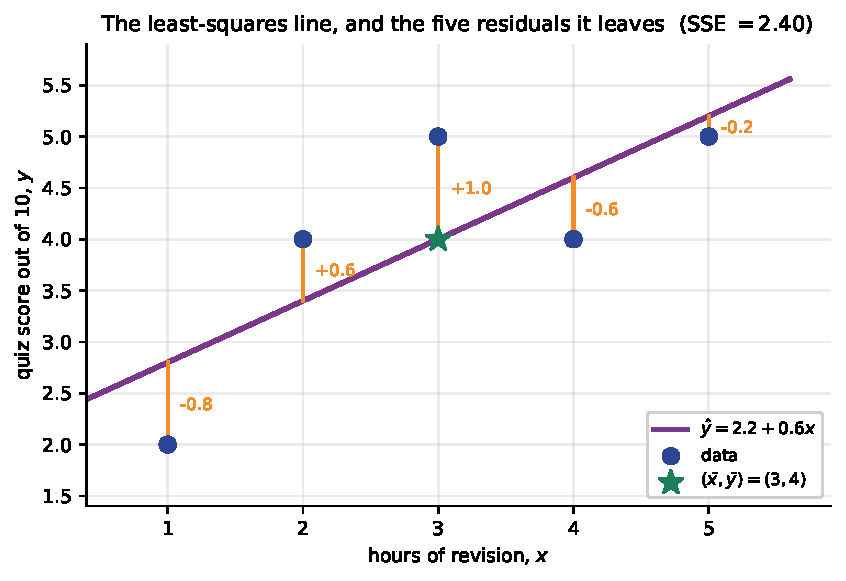
\includegraphics[width=0.72\textwidth]{fitline.pdf}
  \end{center}
  \begin{center}\small
    Orange bars are the residuals: $-0.8, +0.6, +1.0, -0.6, -0.2$. They sum
    to \emph{exactly} zero, and the green star at $(3,4)$ is on the line.
    Neither of those is a coincidence; both are forced by the two normal
    equations.
  \end{center}
\end{frame}

\begin{frame}[shrink=8]{Drawn: least squares is minimising an area}
  \begin{center}
    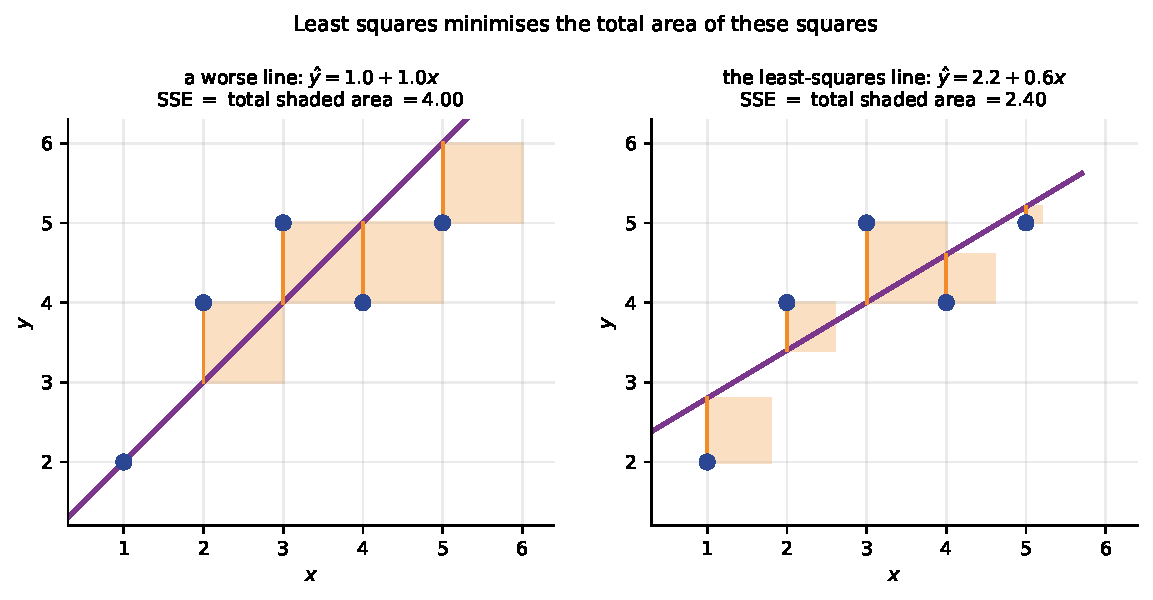
\includegraphics[width=0.90\textwidth]{squares.pdf}
  \end{center}
  \begin{center}\small
    Each residual is drawn as a literal square of side $|e_i|$. The total
    shaded area is the SSE: $4.00$ on the left, $2.40$ on the right.
    \textbf{Least squares slides the line until that total area is as small
    as it can be.}
  \end{center}
\end{frame}

\begin{frame}[shrink=6]{Predict first \#1}
Four candidate lines for the five points. \textbf{Rank them by SSE, and say
which of them have residuals summing to zero.}
  \begin{center}\small
  \begin{tabular}{@{}ll@{}}
    \toprule
    A & $\hat y = 2.0 + 0.7x$\\
    B & $\hat y = 2.2 + 0.6x$\\
    C & $\hat y = 2.5 + 0.5x$\\
    D & $\hat y = 1.0 + 1.0x$\\
    \bottomrule
  \end{tabular}
  \end{center}
\onslide<2->
  \vspace{0.2em}
  \begin{center}\small
  \begin{tabular}{@{}lrrr@{}}
    \toprule
    & \textbf{SSE} & $\sum e_i$ & $\sum x_ie_i$\\
    \midrule
    A: $2.0+0.7x$ & $2.5500$ & $-0.5000$ & $-2.5000$\\
    B: $2.2+0.6x$ & $\mathbf{2.4000}$ & $\mathbf{0.0000}$ & $\mathbf{0.0000}$\\
    C: $2.5+0.5x$ & $2.5000$ & $0.0000$ & $+1.0000$\\
    D: $1.0+1.0x$ & $4.0000$ & $0.0000$ & $-4.0000$\\
    \bottomrule
  \end{tabular}
  \end{center}
\onslide<3->
  \begin{alertblock}{Three of the four have residuals summing to zero}
    \footnotesize \textbf{$\sum e_i = 0$ is necessary, not sufficient.} It is
    only \emph{one} of the two normal equations. B is the only line that also
    satisfies $\sum x_ie_i = 0$, and B is the one with the smallest SSE.
  \end{alertblock}
\end{frame}

\begin{frame}[shrink=8]{Drawn: the four candidates and their scores}
  \begin{center}
    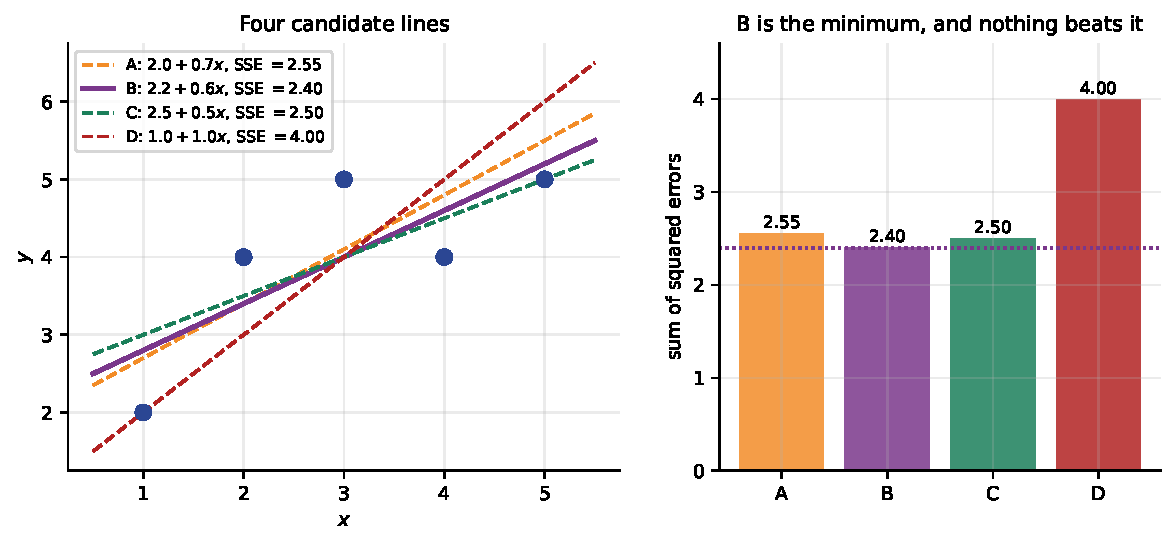
\includegraphics[width=0.94\textwidth]{candidates.pdf}
  \end{center}
  \begin{center}\small
    C is visually almost as good as B and scores $2.50$ against $2.40$. The
    difference is small because we are near the bottom of a bowl, where the
    surface is flat --- which is also why gradient descent takes so long to
    finish the job.
  \end{center}
\end{frame}

\begin{frame}[fragile,shrink=6]{Predict first \#2}
Same five numbers, now through the library. \textbf{To how many decimal
places will \texttt{np.polyfit} and \texttt{LinearRegression} agree with the
hand arithmetic?}
\begin{lstlisting}
p  = np.polyfit(x, y, 1)                       # returns [slope, intercept]
lr = LinearRegression().fit(x.reshape(-1, 1), y)
\end{lstlisting}
\onslide<2->
\begin{outblk}
by hand          b0 = 2.200000000000   b1 = 0.600000000000
np.polyfit       b0 = 2.200000000000   b1 = 0.600000000000
LinearRegression b0 = 2.200000000000   b1 = 0.600000000000
max abs difference, hand vs polyfit          4.441e-16
max abs difference, hand vs LinearRegression 0.000e+00
\end{outblk}
\onslide<3->
\begin{alertblock}{Not ``close''. Identical, to machine precision}
  \footnotesize \texttt{LinearRegression} matched the hand arithmetic
  \textbf{exactly}; \texttt{polyfit} differs in the last bit of a double,
  because it goes through an SVD. \textbf{The library is not doing anything
  you did not just do on paper.} It is doing it faster, and with better
  numerics on larger problems.
\end{alertblock}
\end{frame}

% =====================================================================
\section[Best fit]{The line of best fit and its properties}
\label{sec:props}

\begin{frame}[shrink=5]{Four properties, all free consequences of the derivation}
  \begin{columns}[T]
    \begin{column}{0.49\textwidth}
      \begin{block}{From the first normal equation}
        \small
        \[ \sum_i e_i = 0 \quad\text{and hence}\quad \bar{\hat y} = \bar y. \]
        The residuals cancel exactly. \textbf{Only because an intercept was
        fitted}: that equation is the derivative with respect to $b_0$.
        \[ b_0 = \bar y - b_1\bar x \;\Rightarrow\;
           \hat y(\bar x) = \bar y. \]
        The line passes through the centroid $(\bar x, \bar y)$.
      \end{block}
    \end{column}
    \begin{column}{0.49\textwidth}
      \begin{block}{From the second}
        \small
        \[ \sum_i x_i e_i = 0
           \quad\text{and hence}\quad \sum_i \hat y_i e_i = 0. \]
        The residual vector is orthogonal to the predictor \emph{and} to the
        fitted values --- there is no linear signal left in $e$.
      \end{block}
      \begin{exampleblock}{And the consequence}
        \small
        \[ \underbrace{\sum_i (y_i-\bar y)^2}_{\mathrm{SST}}
           = \underbrace{\sum_i (\hat y_i-\bar y)^2}_{\mathrm{SSR}}
           + \underbrace{\sum_i e_i^2}_{\mathrm{SSE}} \]
        The cross term vanishes \emph{because} of the two facts on the left.
      \end{exampleblock}
    \end{column}
  \end{columns}
\end{frame}

\begin{frame}[fragile,shrink=8]{The properties, on the five points}
\begin{outblk}
  x      y     yhat   residual
  1    2.0    2.80     -0.80
  2    4.0    3.40      0.60
  3    5.0    4.00      1.00
  4    4.0    4.60     -0.60
  5    5.0    5.20     -0.20
sum of residuals        -0.000000000000000
sum of x_i * e_i        -0.000000000000000
sum of yhat_i * e_i     -0.000000000000001
mean of yhat = 4.0000   and ybar = 4.0000
the line at xbar = 3.0 gives 4.0000   and ybar = 4.0000
\end{outblk}
\onslide<2->
\begin{outblk}
SSE (residual)  = 2.4000
SSR (explained) = 3.6000
SST (total)     = 6.0000
SSR + SSE       = 6.0000   and SST = 6.0000
check: SSR = Sxy^2/Sxx = 3.6000
correlation r = Sxy/sqrt(Sxx*Syy) = 0.7746
and b1 = r * sd(y)/sd(x) = 0.7746 * 1.2247/1.5811 = 0.6000
\end{outblk}
\end{frame}

\begin{frame}[fragile,shrink=6]{Drop the intercept and watch the first property die}
Fit $\hat y = b_1 x$ instead. There is now only \emph{one} normal equation,
the one from $\partial/\partial b_1$:
\begin{lstlisting}
b1_noint = np.sum(x * y) / np.sum(x * x)      # fit y = b1 x, no intercept
\end{lstlisting}
\begin{outblk}
no-intercept fit  yhat = 1.2000 x
residuals         [ 0.8  1.6  1.4 -0.8 -1. ]
sum of residuals  +2.0000   (NOT zero)
sum of x_i * e_i  +1.7764e-15   (still zero -- that equation was solved)
SSE               6.8000  against 2.4000 with an intercept
\end{outblk}
\onslide<2->
\begin{alertblock}{The residuals now sum to $+2$, and the SSE nearly trebles}
  \footnotesize $\sum e_i = 0$ was never a law of nature. It is the
  $\partial\,\mathrm{SSE}/\partial b_0 = 0$ equation, and if there is no
  $b_0$ there is no equation. \textbf{Whenever someone tells you residuals
  sum to zero, the words ``with an intercept'' are doing the work.}
\end{alertblock}
\end{frame}

\begin{frame}[shrink=6]{How good is the slope? $S_{xx}$ is the answer}
  Under the four assumptions one can show
  \[
    \mathrm{Var}(b_1) = \frac{\sigma^2}{S_{xx}},
    \qquad
    \mathrm{Var}(b_0) = \sigma^2\left(\frac1n + \frac{\bar x^2}{S_{xx}}\right).
  \]
  \begin{block}{Read the first formula}
    \small $S_{xx}$ is in the denominator, so \textbf{the more spread out
    your $x$ values are, the more precisely you learn the slope}. Doubling
    the spread of $x$ halves the standard error of $b_1$, for free, with the
    same number of rows.
  \end{block}
  \begin{alertblock}{The design lesson}
    \small If you can \emph{choose} where to observe --- an experiment, a
    calibration, a load test --- put your points at the extremes of the
    usable range, not clustered in the middle. Same $n$, better estimate.
  \end{alertblock}
\end{frame}

\begin{frame}[fragile,shrink=8]{Predict first \#3}
$20$ points, noise sd $1.0$, true slope $2.0$. Refit $4000$ times.
\textbf{If I widen the range of $x$ from $\pm 0.5$ to $\pm 4$, what happens
to the spread of the fitted slopes?}
\onslide<2->
\begin{outblk}
half-range of x    Sxx    sd of 4000 fitted slopes   sigma/sqrt(Sxx)
         0.5    1.842                  0.7237            0.7368
         1.0    7.368                  0.3683            0.3684
         2.0   29.474                  0.1859            0.1842
         4.0  117.895                  0.0932            0.0921
\end{outblk}
\onslide<3->
\begin{alertblock}{A factor of $7.8$, from the same $20$ rows}
  \footnotesize Eight times the range of $x$, eight times the precision ---
  because $S_{xx}$ grew $64\times$ and the standard error goes as
  $1/\sqrt{S_{xx}}$. \textbf{The measured column and the theory column agree
  to three decimal places}, so the formula is not decoration.
\end{alertblock}
\end{frame}

\begin{frame}[shrink=8]{Drawn: the same result, twice}
  \begin{center}
    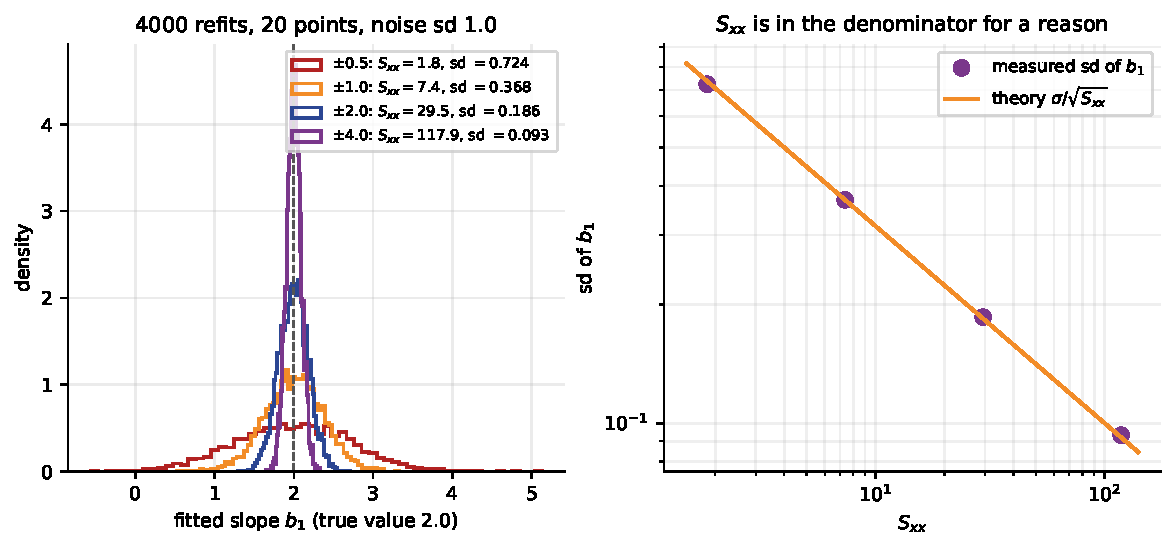
\includegraphics[width=0.94\textwidth]{sxx.pdf}
  \end{center}
  \begin{center}\small
    Left: four sampling distributions of $b_1$, all centred on the true value
    $2.0$ --- least squares is unbiased whatever the spread --- but with very
    different widths. Right: the measured widths against
    $\sigma/\sqrt{S_{xx}}$ on log axes, and they sit on the line.
  \end{center}
\end{frame}

% =====================================================================
\section[Matrix form]{The normal equations in matrix form}
\label{sec:matrix}

\begin{frame}[shrink=5]{The same derivation, written once for any number of columns}
  Stack the data: $X$ is $n \times 2$ with a column of ones, $y$ is
  $n \times 1$, $b = (b_0, b_1)^{\!\top}$.
  \[
    \mathrm{SSE}(b) = \lVert y - Xb\rVert^2
      = (y - Xb)^{\!\top}(y - Xb)
      = y^{\!\top}y - 2b^{\!\top}X^{\!\top}y + b^{\!\top}X^{\!\top}Xb .
  \]
  Differentiate with respect to the vector $b$ and set to zero:
  \[
    \frac{\partial\,\mathrm{SSE}}{\partial b}
      = -2X^{\!\top}y + 2X^{\!\top}Xb = 0
    \qquad\Longrightarrow\qquad
    \boxed{\,X^{\!\top}\!X\,b = X^{\!\top}y\,}
  \]
  \begin{exampleblock}{}
    \centering
    If $X^{\!\top}\!X$ is invertible,
    $\;b = (X^{\!\top}\!X)^{-1}X^{\!\top}y$, and the Hessian is
    $2X^{\!\top}\!X$, positive definite exactly when $X$ has full column
    rank.
  \end{exampleblock}
  \begin{center}\small
    Two scalar equations became one matrix equation, and \textbf{nothing in
    the line above mentions the number of columns}. That is Lecture 11,
    already done.
  \end{center}
\end{frame}

\begin{frame}[shrink=6]{The matrix route on the five points, entirely by hand}
  \[
    X = \begin{pmatrix} 1&1\\1&2\\1&3\\1&4\\1&5 \end{pmatrix},\quad
    X^{\!\top}\!X = \begin{pmatrix} 5 & 15\\ 15 & 55\end{pmatrix},\quad
    X^{\!\top}y = \begin{pmatrix} 20\\ 66 \end{pmatrix}
  \]
  \[
    \det(X^{\!\top}\!X) = 275 - 225 = 50 = n\,S_{xx},
    \qquad
    (X^{\!\top}\!X)^{-1} = \frac{1}{50}
      \begin{pmatrix} 55 & -15\\ -15 & 5\end{pmatrix}
  \]
  \[
    b = \frac{1}{50}\begin{pmatrix} 55 & -15\\ -15 & 5\end{pmatrix}
        \begin{pmatrix} 20\\ 66\end{pmatrix}
      = \frac{1}{50}\begin{pmatrix} 1100 - 990\\ -300 + 330\end{pmatrix}
      = \frac{1}{50}\begin{pmatrix} 110\\ 30\end{pmatrix}
      = \begin{pmatrix} 2.2\\ 0.6\end{pmatrix}
  \]
  \begin{center}\small
    $\sum x_i = 15$, $\sum x_i^2 = 55$, $\sum y_i = 20$,
    $\sum x_iy_i = 2+8+15+16+25 = 66$. \textbf{Four sums, one $2\times2$
    inverse, and the same answer as the scalar formulas.}
  \end{center}
\end{frame}

\begin{frame}[fragile,shrink=6]{And in code, four ways}
\begin{lstlisting}
Xm = np.column_stack([np.ones(n), x])
beta = np.linalg.inv(Xm.T @ Xm) @ (Xm.T @ y)
\end{lstlisting}
\begin{outblk}
X'X =
 [[ 5. 15.]
 [15. 55.]]
X'y = [20. 66.]
det(X'X) = 50.0000   and n*Sxx = 50.0000
inv(X'X) =
 [[ 1.1 -0.3]
 [-0.3  0.1]]
beta = inv(X'X) X'y  = [2.2 0.6]
np.linalg.solve      = [2.2 0.6]
np.linalg.lstsq      = [2.2 0.6]
np.linalg.pinv       = [2.2 0.6]
agrees with the scalar formulas to 2.665e-15
\end{outblk}
\onslide<2->
\begin{center}\small
  $1/50 \times 55 = 1.1$ and $1/50\times(-15) = -0.3$: the printed inverse is
  the fraction you wrote on the board. \textbf{Use \texttt{solve} or
  \texttt{lstsq} in real code, never \texttt{inv}} --- same answer here,
  better numerics when $X^{\!\top}\!X$ is nearly singular.
\end{center}
\end{frame}

% =====================================================================
\section[Two roads]{Two roads to the same answer}
\label{sec:gd}

\begin{frame}[shrink=6]{Lecture 3, revisited with today's model}
  \begin{columns}[T]
    \begin{column}{0.48\textwidth}
      \begin{block}{What L3 did}
        \small
        \[ J(w) = \tfrac1n\lVert Xw - y\rVert^2,\qquad
           \nabla J(w) = \tfrac2n X^{\!\top}(Xw - y) \]
        \[ w \leftarrow w - \eta\,\nabla J(w) \]
        Repeat until it stops moving. Choose $\eta$; hope.
      \end{block}
    \end{column}
    \begin{column}{0.48\textwidth}
      \begin{exampleblock}{What L8 does}
        \small
        \[ \nabla J(w) = 0
           \;\Longrightarrow\;
           X^{\!\top}\!Xw = X^{\!\top}y \]
        \[ w = (X^{\!\top}\!X)^{-1}X^{\!\top}y \]
        One linear solve. No step size, no epochs, no tolerance.
      \end{exampleblock}
    \end{column}
  \end{columns}
  \vspace{0.2em}
  \begin{alertblock}{They are the same objective}
    \small Gradient descent \emph{approaches} the point where the gradient is
    zero. Least squares \emph{solves} for it. The only reason L3 iterated is
    that in general you cannot solve $\nabla J = 0$ in closed form --- and
    for a linear model with squared error, you can.
  \end{alertblock}
\end{frame}

\begin{frame}[fragile,shrink=6]{Predict first \#4}
Gradient descent on $\mathrm{SSE}$ for the five points, from $(0,0)$,
$\eta = 0.01$. \textbf{How many iterations before it matches
$(2.2, 0.6)$ to four decimal places?}
\onslide<2->
\begin{outblk}
 iter        b0        b1        SSE   max|theta-theta*|
    1    0.4000    1.3200     8.2320        1.80e+00
    2    0.3640    1.0680     5.5234        1.84e+00
    5    0.4655    1.0807     5.1381        1.73e+00
   10    0.6072    1.0412     4.7089        1.59e+00
   50    1.3946    0.8231     2.9903        8.05e-01
  200    2.1376    0.6173     2.4035        6.24e-02
 1000    2.2000    0.6000     2.4000        7.44e-08
 4000    2.2000    0.6000     2.4000        1.24e-14
closed form              2.2000    0.6000     2.4000
gradient descent matched the closed form to 4 decimals at iteration 619
\end{outblk}
\onslide<3->
\begin{alertblock}{$\mathbf{619}$ iterations, to reproduce one division}
  \footnotesize And look at the SSE column: after $200$ steps it is
  $2.4035$ against the optimal $2.4000$ --- \textbf{the loss is essentially
  right long before the parameters are}. Near the bottom of a bowl the
  surface is flat, so a large parameter error costs almost no loss. That is
  why $\eta$-tuning felt so fiddly in L3.
\end{alertblock}
\end{frame}

\begin{frame}[shrink=8]{Drawn: the bowl and the descent into it}
  \begin{center}
    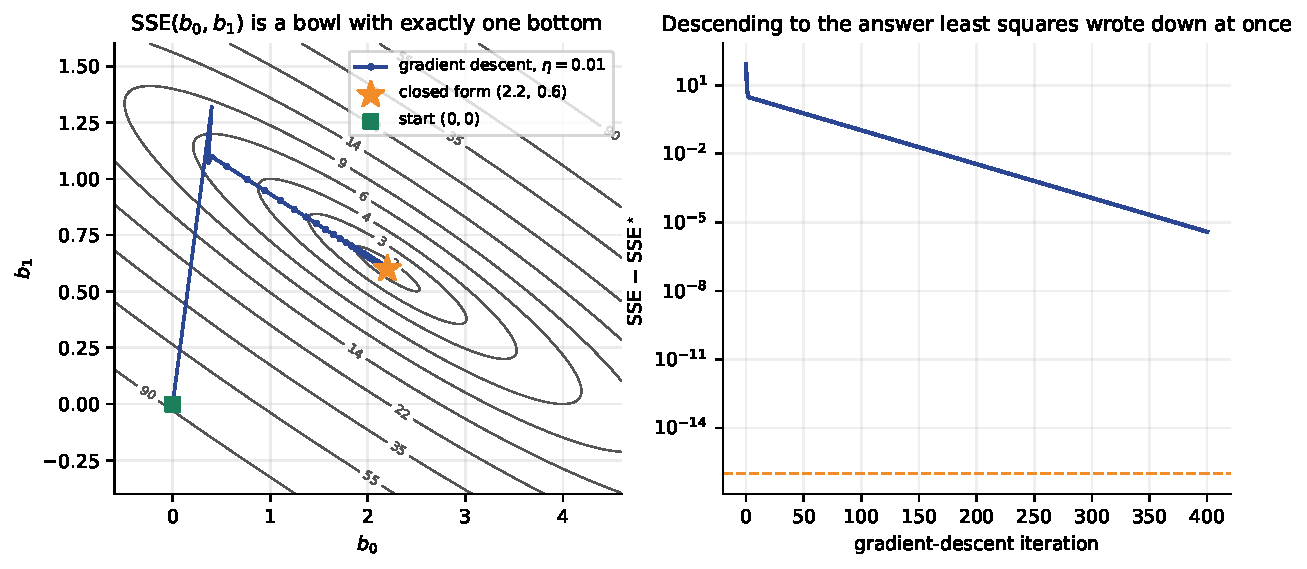
\includegraphics[width=0.94\textwidth]{bowl.pdf}
  \end{center}
  \begin{center}\small
    Left: the SSE contours are ellipses, tilted because $b_0$ and $b_1$ are
    correlated (the $\sum x_i$ off-diagonal of $X^{\!\top}\!X$), so descent
    zig-zags down a valley --- the L6 ravine picture, again. Right: the gap
    to the optimal loss on a log scale. \textbf{The orange star was available
    from the start.}
  \end{center}
\end{frame}

\begin{frame}[fragile,shrink=6]{And on the real data: full-batch, stochastic, exact}
\texttt{load\_diabetes}, \texttt{bmi} against progression, $442$ patients.
Full-batch gradient descent on standardised $x$, then the coefficients
unwound to the original units:
\begin{outblk}
full-batch GD     1 steps   b0 =   30.4267   b1 =  189.8871   J = 20008.2328
full-batch GD    10 steps   b0 =  135.7983   b1 =  847.4904   J = 4180.8086
full-batch GD   100 steps   b0 =  152.1335   b1 =  949.4353   J = 3890.4566
full-batch GD  2000 steps   b0 =  152.1335   b1 =  949.4353   J = 3890.4566
closed form               b0 =  152.1335   b1 =  949.4353   J = 3890.4566
difference in the slope   4.547e-13 (relative 4.441e-16)
SGDRegressor (stochastic) b0 =  149.5577   b1 =  891.1257   J = 3904.7835
\end{outblk}
\onslide<2->
\begin{alertblock}{Full-batch arrives exactly; stochastic stops $6.1\%$ short}
  \footnotesize $100$ steps of full-batch descent reproduce
  $(X^{\!\top}\!X)^{-1}X^{\!\top}y$ to $13$ decimal places.
  \texttt{SGDRegressor} with a constant step lands $6.1\%$ away on the slope
  --- \textbf{that is the L3 noise floor, not a bug}: a constant-step
  stochastic method converges to a \emph{region}, not a point.
\end{alertblock}
\end{frame}

\begin{frame}[shrink=6]{So when do you use which?}
  \begin{center}\small
  \begin{tabular}{@{}lll@{}}
    \toprule
    & \textbf{Closed form} & \textbf{Gradient descent}\\
    \midrule
    Cost & $O(nd^2 + d^3)$, one pass & $O(nd)$ per step, many steps\\
    Memory & needs $X^{\!\top}\!X$, or all of $X$ & one mini-batch at a
      time\\
    Tuning & none & step size, schedule, batch size, stopping\\
    Answer & exact & as close as you can afford\\
    Fails when & $d$ large, $X^{\!\top}\!X$ singular & almost never, slowly\\
    Extends to & squared loss on a linear model & anything differentiable\\
    \bottomrule
  \end{tabular}
  \end{center}
  \vspace{0.2em}
  \begin{alertblock}{Rule of thumb}
    \small Small $d$ (say under a few thousand columns) and the data fits in
    memory: \textbf{use the closed form}, which is what
    \texttt{LinearRegression} does. Huge $n$, huge $d$, streaming data, or a
    model that is not linear-with-squared-loss: \textbf{descend}.
  \end{alertblock}
  \begin{center}\small
    Logistic regression, two lectures away, has \emph{no} closed form. That
    is why L3 came first.
  \end{center}
\end{frame}

% =====================================================================
\section[Cautions]{What least squares will not tell you}
\label{sec:caution}

\begin{frame}[fragile,shrink=6]{Predict first \#5}
Take the five points and move \emph{one} $y$ value from $5$ to $9$.
\textbf{Does it matter which one? Move the point at $x=3$, then the point at
$x=5$. Which change moves the slope more?}
\onslide<2->
\begin{outblk}
point moved         b0       b1    change in b1
none                2.2000   0.6000        +0.0000
y at x=3: 5 -> 9    3.0000   0.6000        +0.0000
y at x=5: 5 -> 9    0.6000   1.4000        +0.8000
y at x=1: 2 -> -2  -1.0000   1.4000        +0.8000
leverage (x-xbar)^2/Sxx: [0.4 0.1 0.  0.1 0.4]
\end{outblk}
\onslide<3->
\begin{alertblock}{The middle point cannot change the slope. At all}
  \footnotesize Its leverage is \textbf{exactly zero}, because
  $x_3 = \bar x$ and $b_1 = \sum (x_i-\bar x)(y_i-\bar y)/S_{xx}$ weights
  each row by $(x_i - \bar x)$. Move it anywhere you like: only $b_0$
  responds. The two end points carry $0.4$ of the leverage each ---
  \textbf{four points out of five hold $80\%$ of the influence}.
\end{alertblock}
\end{frame}

\begin{frame}[shrink=8]{Drawn: same size of change, different consequence}
  \begin{center}
    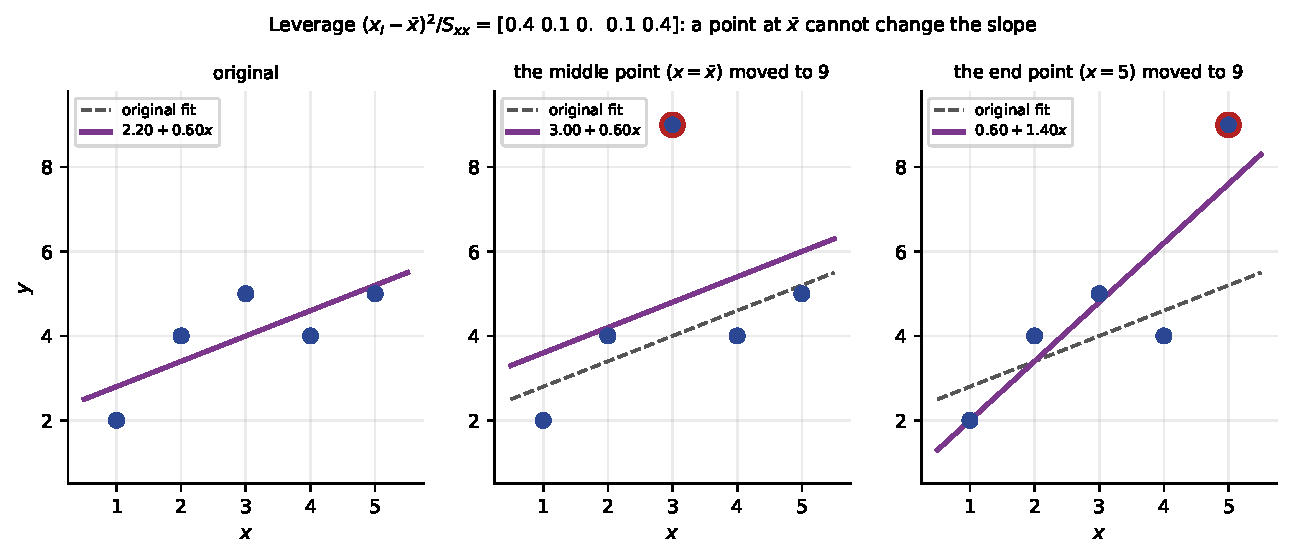
\includegraphics[width=0.98\textwidth]{leverage.pdf}
  \end{center}
  \begin{center}\small
    The same $+4$ error in $y$. In the middle panel the line lifts and keeps
    its slope; in the right panel it pivots. \textbf{``Is this an outlier?''
    is the wrong question --- ask where it sits in $x$.}
  \end{center}
\end{frame}

\begin{frame}[fragile,shrink=8]{Predict first \#6 --- Anscombe's quartet}
Four datasets, eleven points each. Their means, $S_{xx}$, $S_{xy}$, fitted
lines and SSE are printed below. \textbf{Before you look at the next slide:
how similar do you expect the four scatterplots to be?}
\onslide<2->
\begin{outblk}
set   xbar   ybar     Sxx     Sxy      b0      b1      SSE
I      9.00   7.50   110.00   55.01  3.0001  0.5001  13.7627
II     9.00   7.50   110.00   55.00  3.0009  0.5000  13.7763
III    9.00   7.50   110.00   54.97  3.0025  0.4997  13.7562
IV     9.00   7.50   110.00   54.99  3.0017  0.4999  13.7425
\end{outblk}
\onslide<3->
\begin{center}\small
  Every column agrees to two decimal places. \textbf{Four datasets,
  indistinguishable by every number least squares computes.}
\end{center}
\end{frame}

\begin{frame}[shrink=8]{Drawn: and here they are}
  \begin{center}
    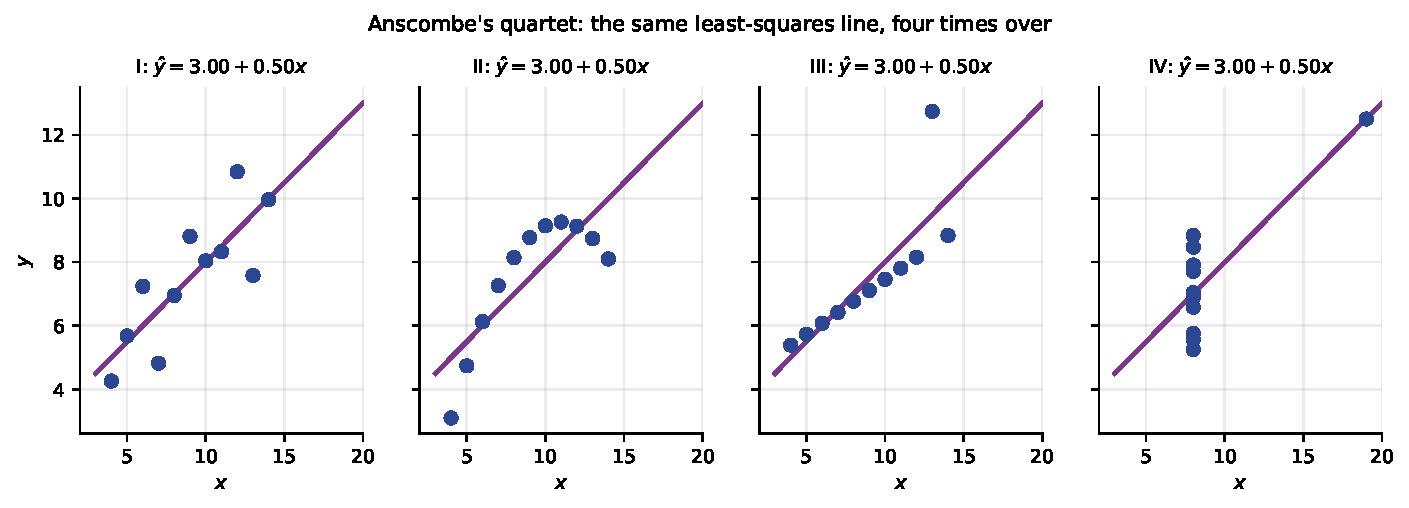
\includegraphics[width=0.99\textwidth]{anscombe.pdf}
  \end{center}
  \begin{alertblock}{The estimates were never the point on their own}
    \footnotesize I is a reasonable linear fit. II is a \textbf{parabola} and
    the model is wrong. III is a perfect line plus \textbf{one} bad point.
    IV has ten points at $x=8$ and one point at $x=19$ that \emph{alone}
    determines the slope --- leverage $= 1.0$. \textbf{Always plot the data,
    and always plot the residuals.} That is Lecture 9.
  \end{alertblock}
\end{frame}

\begin{frame}[fragile,shrink=7]{One more thing least squares will not tell you}
Every single-predictor regression on \texttt{load\_diabetes}, ranked by SSE:
\begin{outblk}
feature        b1        b0        SSE      corr(x,y)
bmi         949.435   152.133   1719581.8      0.5865
s5          916.137   152.133   1781701.4      0.5659
bp          714.738   152.133   2110158.3      0.4415
...
sex          69.715   152.133   2616148.9      0.0431
total sum of squares about ybar: 2621009.1
\end{outblk}
\onslide<2->
\begin{center}\small
  \textbf{Every intercept is $152.133$}, because $b_0 = \bar y - b_1\bar x$
  and every column of this dataset is already centred, so $\bar x = 0$. The
  best single predictor removes $34\%$ of the total sum of squares; the worst
  removes $0.2\%$.
\end{center}
\onslide<3->
\begin{center}\small
  And none of this is causation. \texttt{bmi} predicting progression is a
  statement about \emph{this table}, not about what happens if you change a
  patient's BMI.
\end{center}
\end{frame}

% =====================================================================
\section{Summary}
\label{sec:summary}

\begin{frame}[shrink=15]{Summary --- twelve lines}
  \begin{enumerate}\small
    \item Regression models a quantitative $y$ as a systematic part plus
      noise: $y = f(x) + \varepsilon$. Two jobs --- prediction and
      explanation --- and you must say which.
    \item A model is \textbf{linear} when it is linear in the
      \emph{parameters}. A parabola is a linear model; $\beta_0 +
      \beta_0\beta_1x$ is not.
    \item Eight steps: problem, variables, data, specification, method, fit,
      validation, use. Steps 1--3 decide the analysis.
    \item Least squares minimises $\mathrm{SSE}(b_0,b_1) = \sum(y_i - b_0 -
      b_1x_i)^2$. Squares because the criterion is differentiable and its
      derivative is \emph{linear} in the unknowns.
    \item Setting both partials to zero gives the \textbf{normal equations},
      and solving them gives
      $b_1 = S_{xy}/S_{xx}$, $b_0 = \bar y - b_1\bar x$.
    \item The Hessian is $2\bigl(\begin{smallmatrix} n & \sum x_i\\
      \sum x_i & \sum x_i^2\end{smallmatrix}\bigr)$ with
      $\det = 4nS_{xx} > 0$: a strict, unique, global minimum.
    \item Five points, $S_{xx}=10$, $S_{xy}=6$: $\hat y = 2.2 + 0.6x$,
      SSE $=2.40$. \texttt{np.polyfit} agrees to $4\times10^{-16}$;
      \texttt{LinearRegression} to $0$.
    \item Matrix form: $X^{\!\top}\!Xb = X^{\!\top}y$, and by hand
      $\frac1{50}\bigl(\begin{smallmatrix}55&-15\\-15&5\end{smallmatrix}
      \bigr)\bigl(\begin{smallmatrix}20\\66\end{smallmatrix}\bigr)
      = (2.2, 0.6)$.
    \item With an intercept, $\sum e_i = 0$ and the line passes through
      $(\bar x, \bar y)$. Drop the intercept and $\sum e_i$ became $+2.0$.
      $\sum e_i = 0$ is necessary but \textbf{not sufficient}: three of four
      candidate lines had it.
    \item Gradient descent on the same objective took \textbf{619 iterations}
      to match one division, and on diabetes reproduced
      $(X^{\!\top}\!X)^{-1}X^{\!\top}y$ to $4\times10^{-16}$ relative.
      Stochastic descent stopped $6.1\%$ short.
    \item $\mathrm{Var}(b_1) = \sigma^2/S_{xx}$: widening the range of $x$
      eightfold cut the spread of the slope by $7.8\times$, on the same $20$
      rows.
    \item \textbf{Anscombe's quartet}: four datasets with the same
      $\bar x, \bar y, S_{xx}, S_{xy}, b_0, b_1$ and SSE, and four completely
      different pictures.
  \end{enumerate}
\end{frame}

\begin{frame}[shrink=3]{Before the next lecture}
  \begin{columns}[T]
    \begin{column}{0.48\textwidth}
      \begin{block}{Read}
        \texttt{notes.pdf} --- the derivation written out with every step,
        the matrix version, the proof that the cross term vanishes, and
        \textbf{10 practice questions with full worked solutions}.
      \end{block}
      \begin{block}{Do}
        Questions 1, 2 and 7. Questions 1 and 2 are by-hand least-squares
        computations of exactly the kind the test will ask; question 7 is
        the derivation, from scratch, on a blank page.
      \end{block}
    \end{column}
    \begin{column}{0.48\textwidth}
      \begin{exampleblock}{Next: maximum likelihood and adequacy}
        Where does squared error \emph{come from}? Assume Normal noise, write
        the likelihood, maximise it --- and get today's estimator back.
        Then $R^2$, residual diagnostics and over-fitting.
      \end{exampleblock}
      \begin{alertblock}{Carry one number across}
        $\mathrm{SSR}/\mathrm{SST} = 3.6/6.0 = 0.6$ on the five points, and
        $r^2 = 0.7746^2 = 0.6$ as well. \textbf{That is not a coincidence,
        and Lecture 9 gives it a name.}
      \end{alertblock}
    \end{column}
  \end{columns}
  \begin{center}
    \small Materials: \texttt{\AMLRepoURL}
  \end{center}
  \slidesources{\AMLUnitVSources}
\end{frame}

\end{document}
